\section{Laboratory work implementation}

\subsection{Tasks and Points}

\begin{itemize}
	\item Basic Level (nota 5 || 6) :
	\begin{itemize}
		\item conecteaza-te la server folosind SSH
		\item compileaza cel putin 2 sample programs din setul HelloWolrdPrograms folosind CLI
		\item executa primul commit folosind VCS
	\end{itemize}
	\item Normal Level (nota 7 || 8):
	\begin{itemize}
		\item initializeaza un nou repositoriu
		\item configureaza-ti VCS
		\item crearea branch-urilor (creeaza cel putin 2 branches)
		\item commit pe ambele branch-uri (cel putin 1 commit per branch)
	\end{itemize}
	\item Advanced Level (nota 9 || 10):
	\begin{itemize}
		\item seteaza un branch to track a remote origin pe care vei putea sa faci push (ex. Github, Bitbucket or custom server)
		\item reseteaza un branch la commit-ul anterior
		\item merge 2 branches
	\item conflict solving between 2 branches
	\end{itemize}
	\end{itemize}

\subsection{Analiza lucrarii de laborator}
Pentru inceput am reusit sa creez un repositoriu pe github , creind un repozitoriu, dupa care am instalat programul git in calculator.
Am reusit sa conectez folosind SSH prin git remote add origin email.
Am creeat o cheia ce ma autorizeaza automat prin  ssh-keygen care creeaza un passphrase for key pentru autentificarea de la acest device.
\begin{center}
	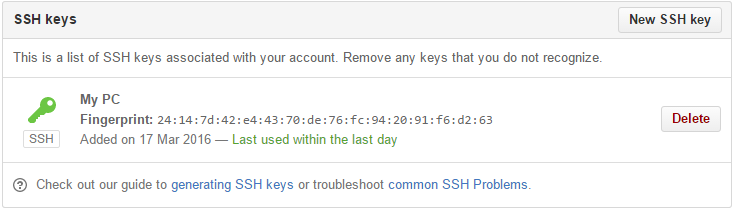
\includegraphics[width=0.7\linewidth]{1key}
\end{center}
Am creeat un file java si dupa instalara jdk-ului in windowsul local, am reusit sa compilez acest cod prin ssh in github, prin javac - compilarea si accesarea file-ului compilat (Avem necesitatea stricta de a instala virtual masina in windows-ul local pentru posibilitatea rularii programelor, pe motiv ca se acceseaza acest jdk din calculatorul meu).
\begin{center}
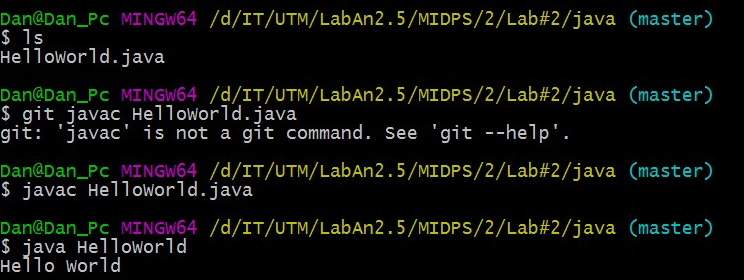
\includegraphics[width=0.7\linewidth]{2java}
\end{center}

Am reusti sa comentez fiecare schimbare in file-urile locale prin comenzile add dupa care comentem prin commit -m "comentariu" si git push, care introduce schimbarile pe git. Afisarea comentariilor:
\begin{center}

\includegraphics[width=0.7\linewidth]{3commit}
\end{center}

Initializarea unui nou repozitoriu prin comanda init prin ssh si am configurat setarile lui
\begin{center}
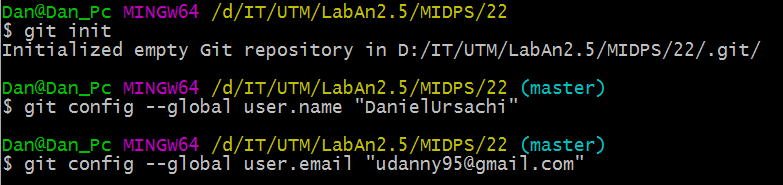
\includegraphics[width=0.7\linewidth]{4repozitoriu}
\end{center}
Dupa care in https://github.com/new am introdus acest repozitoriu si l-am adaugat
\begin{center}
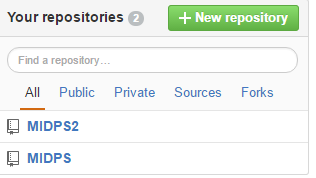
\includegraphics[width=0.5\linewidth]{5repozGit}
\end{center}
Am creat un branch nou prin ssh cu denumirea Samurai si l-am ales pentru prelucrarea schimbarilor prin el
\begin{center}
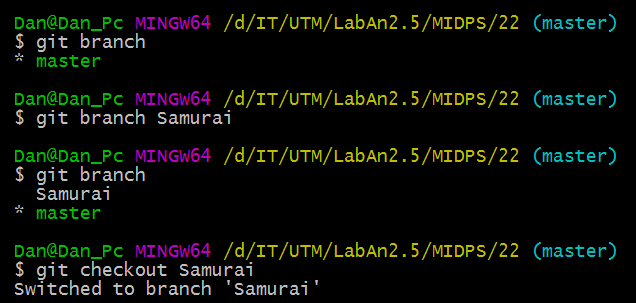
\includegraphics[width=0.7\linewidth]{6branch1}
\end{center}
Am efectuat efectuat o actiune prin acest branch nou
\begin{center}
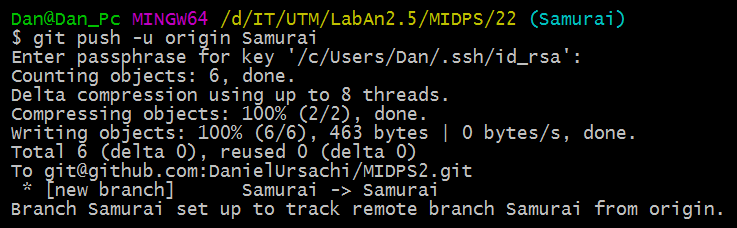
\includegraphics[width=0.7\linewidth]{7branch2}
\end{center}
Dupa care am reusit sa fac commit prin branch-ul nou si in calitate de master trebuie sa acceptam sau nu schimbarile
\begin{center}
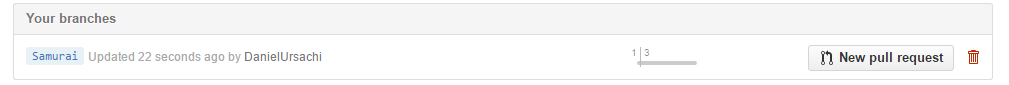
\includegraphics[width=0.7\linewidth]{8request}
\end{center}
Prin acceptare, obtinem:
\begin{center}

\includegraphics[width=0.7\linewidth]{9accept}
\end{center}
Crearea si alegerea unui nou branch
\begin{center}
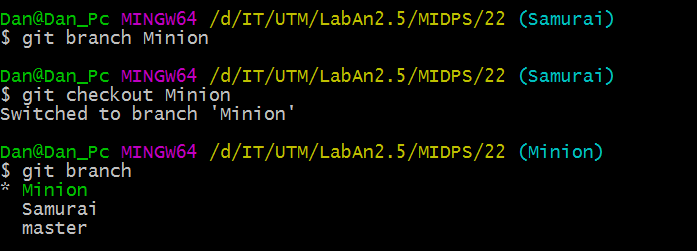
\includegraphics[width=0.7\linewidth]{10branch2}
\end{center}
Obtinem:
\begin{center}
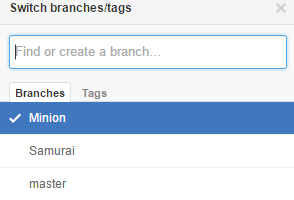
\includegraphics[width=0.5\linewidth]{11branch2git}
\end{center}
Compilarea file-ului 2
\begin{center}
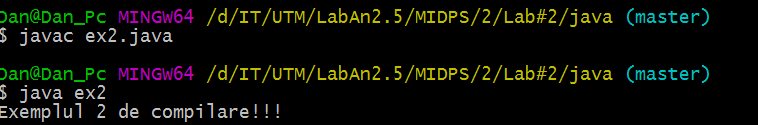
\includegraphics[width=0.7\linewidth]{12java2}
\end{center}
Rularea programului de C prin metoda similara la Java
\begin{center}
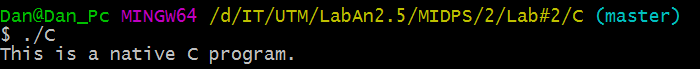
\includegraphics[width=0.7\linewidth]{13C}
\end{center}
Am creeat un file gol .txt, dupa care prin cele 2 branchuri, prin branch-ul Samurai am scris in file "Samurai:aaaa" si prin branch-ul Minion am scris in file "Minion:bbbbb", dupa care schimbind branch-ul in master, prin apelarea functiei ce ne afiseaza commit-urile, am obtinut CONFLICTUL:
\begin{center}
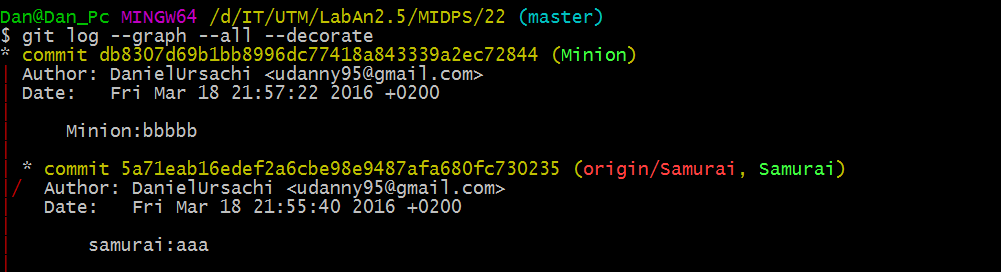
\includegraphics[width=0.7\linewidth]{14conflict}
\end{center}
Pentru rezolvarea conflictului am ales schimbarile branch-ului Samurai prin comanda:
\begin{center}
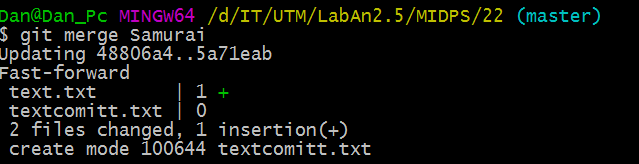
\includegraphics[width=0.7\linewidth]{15rezolv}
\end{center}
Astfel, am obtinut prin branch-ul master continutul file-ului echivalent cu cel al branch-ului Samurai
\begin{center}

\includegraphics[width=0.5\linewidth]{16demonstratie}
\end{center}
RESETAREA branch-ului la comitul anterior am efectuat prin schimbarea a 2 schimbari a textului din file din acelasi branch
\begin{center}
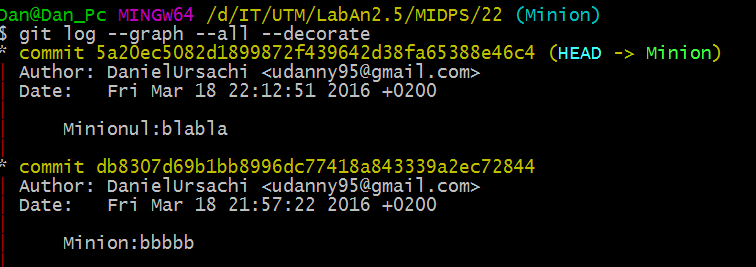
\includegraphics[width=0.7\linewidth]{17resetare}
\end{center}
Dupa care, selectam prima parte a adresa codului pentru schimbare si o setam la checkout:
\begin{center}
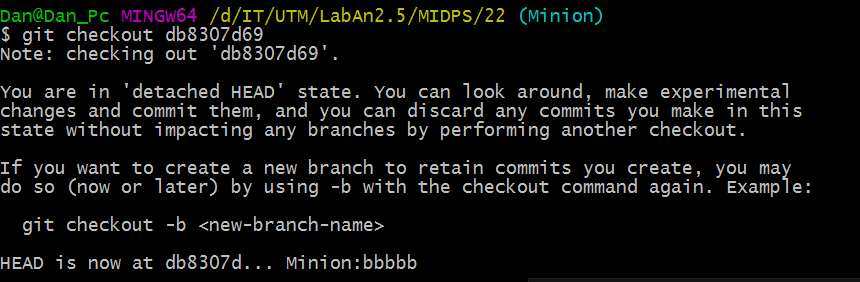
\includegraphics[width=0.7\linewidth]{18resetarechiar}
\end{center}











\clearpage